% article_FR_3.0.tex — one-page presentation of WAC 3.0 for a DFIR magazine,
% French edition. The English edition is article_EN_3.0.tex, in this folder:
% both are maintained together, paragraph for paragraph. It follows the article
% on version 2.0 (article_FR_2.0.tex) and presents only what 3.0 adds.
%
% Build (LuaLaTeX, as the editor's recipe; build artefacts removed after):
%     ../build-docs.sh article/article_FR_3.0.tex
%
% Every figure comes from the comparison, validation and harmlessness files
% (doc/comparison, doc/validation, doc/harmlessness), measured on 29 and 30
% October 2026 on version 3.0.0. Backlog B-058.

\documentclass[10pt,a4paper,twocolumn]{article}
\usepackage[french]{babel}
\usepackage{fontspec}
\setmainfont{Noto Sans}
\setmonofont{DejaVu Sans Mono}[Scale=0.84]
\usepackage[top=13mm,bottom=13mm,left=14mm,right=14mm,columnsep=7mm]{geometry}
\usepackage{xcolor}
\usepackage{titlesec}
\usepackage{enumitem}
\usepackage{array}
\usepackage{graphicx}
\usepackage{caption}
\captionsetup{font={small,color=gris},skip=2pt}
\usepackage[hidelinks]{hyperref}
\definecolor{marine}{HTML}{0A1A33}
\definecolor{bleu}{HTML}{2F6DB5}
\definecolor{gris}{HTML}{5B6573}
\pagestyle{empty}
\setlength{\parindent}{0pt}
\setlength{\parskip}{0.35em}
\titleformat{\section}{\color{marine}\normalsize\bfseries}{}{0em}{}
\titlespacing*{\section}{0pt}{0.7em}{0.2em}
\setlist{nosep,leftmargin=1.1em}
\newcommand{\wac}{\textsc{wac}}
\newcommand{\fichier}[1]{\texttt{#1}}
\hypersetup{pdftitle={WAC 3.0 — de Windows XP à Windows 11, et ce que le disque a gardé}}

\begin{document}

\twocolumn[{%
  {\color{marine}\LARGE\bfseries WAC 3.0 : de Windows XP à Windows 11, et ce que le disque a gardé}\par
  \vspace{0.3em}
  {\color{gris}Centre d'Excellence Cyberdéfense Aérospatiale (CEC), École de l'air et de l'espace}\par
  \vspace{0.6em}
  {\itshape L'article consacré à la version 2.0 présentait \wac{} (Windows
  Artefacts Collector) : un collecteur libre, en C++, qui lit les volumes en
  brut, convertit en JSON sur le poste d'analyse, scelle et journalise chacune
  de ses opérations, sans rien écrire sur la machine examinée. La version 3.0
  garde ces principes et étend leur portée : tous les postes Windows depuis
  XP~SP1, les clichés instantanés lus sans le service VSS, les fichiers
  supprimés, et onze artefacts de plus.}\par
  \vspace{0.9em}
}]

\section{Tous les postes, de XP à 11}
Un second exécutable, \fichier{WAC32.exe}, construit sur les mêmes sources,
collecte de Windows~XP~SP1 à Windows~8 en 32~bits ; \fichier{WAC.exe} reste
celui de toutes les versions 64~bits. Chaque version a ses formats, et
\wac{} les décode : Prefetch et ShimCache de XP à 8.1, files BITS,
\fichier{Thumbs.db}, dépôt WMI et journaux \fichier{.evt} de XP. Une table des artefacts par version décide de ce qui se
prend : un artefact absent d'une version n'est pas cherché ; une source qui
devrait être là et ne l'est pas est déclarée « attendue et introuvable » ---
cette absence est un constat ; un format sans décodeur est prélevé brut et
dit « non pris en charge », jamais rendu comme une liste vide.

\section{Les clichés instantanés, sans VSS}
Les ruches, journaux et fichiers tels que chaque cliché instantané les a
gardés sont relus depuis le volume lui-même, en brut : aucun appel au service
VSS, aucune écriture sur le disque examiné. Ce qu'un cliché garde et que le
volume n'a plus est signalé --- une valeur Run effacée depuis, un événement
d'un journal vidé.

\section{Les fichiers supprimés}
Trois niveaux, réglés dans \fichier{wac.yml} : le contenu des
enregistrements libres de la \fichier{\$MFT} ; les noms restés dans l'espace
libre des index de répertoires ; à la demande, les fichiers PE, ZIP et PDF
taillés dans l'espace libre, à leur taille exacte. Les volumes FAT et exFAT des
clés USB sont lus de même. Chaque fichier récupéré entre dans la consigne avec
ses empreintes ; sur un SSD, ce que TRIM a effacé ne se rend plus. Sur la machine de test, le niveau par défaut en récupère
12\,529 (4,3~Go) en 156~s.

\section{Onze artefacts de plus}
L'index de recherche de Windows (\fichier{Windows.edb}), Sysmon (configuration,
archives) et les journaux déplacés, les profils PowerShell, Entra ID, OneDrive,
les fichiers ETW, Defender for Endpoint, le journal du pare-feu, les secteurs
de démarrage (MBR, GPT, partition EFI), les journaux d'Intune : 80 artefacts
au lieu de 69. Les manuels confrontent cette collecte à MITRE ATT\&CK : sur les
479 techniques Windows de la version~20.0, 475 laissent une trace que \wac{}
prélève --- 463 dans les journaux et sur le disque, 7 dans les journaux seuls,
5 sur le disque seul ; 4 n'en laissent aucune.

\section{La procédure, renforcée}
Le sceau du manifeste s'affiche en fin de collecte, à reporter au
procès-verbal, et les scripts livrés lui opposent le manifeste. Une revue de code et
de sécurité de tout le projet a précédé la publication.

\section{Aucune trace, remesurée}
Sur le clone figé de la machine de test, sous Sysmon, chaque outil est relancé
depuis une clé. \wac{} n'écrit toujours \textbf{aucun fichier} sur C: et
\textbf{aucune valeur de registre} ; les ruches, relues hors ligne et
confrontées clé par clé à l'état figé, le confirment. La mesure a relevé une
trace, corrigée depuis : la liste des modules de chaque processus faisait
ouvrir 42 processus en accès complet par Windows ; ils le sont désormais en
requête et lecture mémoire seules. KAPE et ses modules, dans les mêmes
conditions, écrivent dans la ruche de l'utilisateur, créent 8 clés de traçage
dans SOFTWARE et 28 fichiers sur C:.

\section{Des tests sur chaque version}
Le cycle autonome tourne sous Windows~XP, Vista, 7, 8, 8.1 et 11. Sous
Windows~11, il passe 553 contrôles, chacun contre une source indépendante ;
les onze outils d'Eric Zimmerman, confrontés de nouveau sur les mêmes pièces,
donnent les mêmes valeurs que \wac{}, ou des valeurs fausses (SrumECmd décale
huit lignes, AmcacheParser invente 5\,500 valeurs).

\section{En chiffres}
\begin{tabular}{@{}>{\raggedright\arraybackslash}p{0.72\columnwidth}@{\hspace{0.5em}}r@{}}
Artefacts prélevés (2.0 : 69) & 80 \\
Versions de Windows & XP~SP1 à 11 \\
Collecte hors exécutables et fichiers supprimés (KAPE : 53~s) & 64~s \\
Fichiers supprimés récupérés, machine de test & 12\,529 \\
Fichiers écrits sur C: par \wac{} & 0 \\
Contrôles du cycle Windows~11 & 553 \\
Techniques ATT\&CK Windows couvertes & 475 / 479 \\
\end{tabular}

\section{Disponibilité}
Version 3.0.0, Windows~XP~SP1 à 11 (x86 et x64), licence GPL~3.0 :
\url{https://github.com/dev-cec/WAC}. Manuels, dossiers de validation,
d'innocuité et de comparaison en français et en anglais, mesures des 29 et
30 octobre 2026.

\vfill
\begin{center}
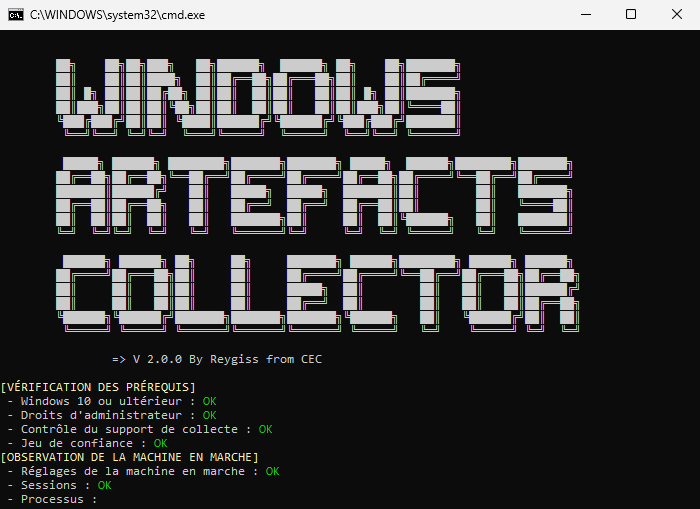
\includegraphics[width=\columnwidth,height=30mm,keepaspectratio]{../images/wac-running_FR.png}
\captionof*{figure}{\wac{} en cours de collecte.}
\end{center}

\end{document}
